% (find-LATEX "2020-2-C3-MT2.tex")
% (defun c () (interactive) (find-LATEXsh "lualatex -record 2020-2-C3-MT2.tex" :end))
% (defun C () (interactive) (find-LATEXsh "lualatex 2020-2-C3-MT2.tex" "Success!!!"))
% (defun D () (interactive) (find-pdf-page      "~/LATEX/2020-2-C3-MT2.pdf"))
% (defun d () (interactive) (find-pdftools-page "~/LATEX/2020-2-C3-MT2.pdf"))
% (defun e () (interactive) (find-LATEX "2020-2-C3-MT2.tex"))
% (defun o () (interactive) (find-LATEX "2020-2-C3-MT2.tex"))
% (defun u () (interactive) (find-latex-upload-links "2020-2-C3-MT2"))
% (defun v () (interactive) (find-2a '(e) '(d)))
% (defun d0 () (interactive) (find-ebuffer "2020-2-C3-MT2.pdf"))
% (defun cv () (interactive) (C) (ee-kill-this-buffer) (v) (g))
%          (code-eec-LATEX "2020-2-C3-MT2")
% (find-pdf-page   "~/LATEX/2020-2-C3-MT2.pdf")
% (find-sh0 "cp -v  ~/LATEX/2020-2-C3-MT2.pdf /tmp/")
% (find-sh0 "cp -v  ~/LATEX/2020-2-C3-MT2.pdf /tmp/pen/")
%     (find-xournalpp "/tmp/2020-2-C3-MT2.pdf")
%   file:///home/edrx/LATEX/2020-2-C3-MT2.pdf
%               file:///tmp/2020-2-C3-MT2.pdf
%           file:///tmp/pen/2020-2-C3-MT2.pdf
% http://angg.twu.net/LATEX/2020-2-C3-MT2.pdf
% (find-LATEX "2019.mk")
% (find-CN-aula-links "2020-2-C3-MT2" "3" "c3m202mt2" "c3mt2")
%
% Video:
% (find-ssr-links "c3m202mt2" "2020-2-C3-MT2")
% (code-video     "c3m202mt2video" "$S/http/angg.twu.net/eev-videos/2020-2-C3-MT2.mp4")
% (find-c3m202mt2video "0:00")

% «.defs»	(to "defs")
% «.title»	(to "title")
% «.regras»	(to "regras")
% «.dicas»	(to "dicas")
% «.video»	(to "video")
%
% «.djvuize»	(to "djvuize")

\documentclass[oneside,12pt]{article}
\usepackage[colorlinks,citecolor=DarkRed,urlcolor=DarkRed]{hyperref} % (find-es "tex" "hyperref")
\usepackage{amsmath}
\usepackage{amsfonts}
\usepackage{amssymb}
\usepackage{pict2e}
\usepackage[x11names,svgnames]{xcolor} % (find-es "tex" "xcolor")
\usepackage{colorweb}                  % (find-es "tex" "colorweb")
%\usepackage{tikz}
%
% (find-dn6 "preamble6.lua" "preamble0")
%\usepackage{proof}   % For derivation trees ("%:" lines)
%\input diagxy        % For 2D diagrams ("%D" lines)
%\xyoption{curve}     % For the ".curve=" feature in 2D diagrams
%
\usepackage{edrx15}               % (find-LATEX "edrx15.sty")
\input edrxaccents.tex            % (find-LATEX "edrxaccents.tex")
\input edrxchars.tex              % (find-LATEX "edrxchars.tex")
\input edrxheadfoot.tex           % (find-LATEX "edrxheadfoot.tex")
\input edrxgac2.tex               % (find-LATEX "edrxgac2.tex")
%
%\usepackage[backend=biber,
%   style=alphabetic]{biblatex}            % (find-es "tex" "biber")
%\addbibresource{catsem-slides.bib}        % (find-LATEX "catsem-slides.bib")
%
% (find-es "tex" "geometry")
\usepackage[a6paper, landscape,
            top=1.5cm, bottom=.25cm, left=1cm, right=1cm, includefoot
           ]{geometry}
%
\begin{document}

%\catcode`\^^J=10
%\directlua{dofile "dednat6load.lua"}  % (find-LATEX "dednat6load.lua")

% %L dofile "edrxtikz.lua"  -- (find-LATEX "edrxtikz.lua")
% %L dofile "edrxpict.lua"  -- (find-LATEX "edrxpict.lua")
% \pu

% «defs»  (to ".defs")
% (find-LATEX "edrx15.sty" "colors-2019")
\long\def\ColorRed   #1{{\color{Red1}#1}}
\long\def\ColorViolet#1{{\color{MagentaVioletLight}#1}}
\long\def\ColorViolet#1{{\color{Violet!50!black}#1}}
\long\def\ColorGreen #1{{\color{SpringDarkHard}#1}}
\long\def\ColorGreen #1{{\color{SpringGreenDark}#1}}
\long\def\ColorGreen #1{{\color{SpringGreen4}#1}}
\long\def\ColorGray  #1{{\color{GrayLight}#1}}
\long\def\ColorGray  #1{{\color{black!30!white}#1}}
\long\def\ColorBrown #1{{\color{Brown}#1}}
\long\def\ColorBrown #1{{\color{brown}#1}}
\long\def\ColorOrange#1{{\color{orange}#1}}

\long\def\ColorShort #1{{\color{SpringGreen4}#1}}
\long\def\ColorLong  #1{{\color{Red1}#1}}

\def\frown{\ensuremath{{=}{(}}}
\def\True {\mathbf{V}}
\def\False{\mathbf{F}}
\def\D    {\displaystyle}

\def\drafturl{http://angg.twu.net/LATEX/2020-2-C3.pdf}
\def\drafturl{http://angg.twu.net/2020.2-C3.html}
\def\draftfooter{\tiny \href{\drafturl}{\jobname{}} \ColorBrown{\shorttoday{} \hours}}



%  _____ _ _   _                               
% |_   _(_) |_| | ___   _ __   __ _  __ _  ___ 
%   | | | | __| |/ _ \ | '_ \ / _` |/ _` |/ _ \
%   | | | | |_| |  __/ | |_) | (_| | (_| |  __/
%   |_| |_|\__|_|\___| | .__/ \__,_|\__, |\___|
%                      |_|          |___/      
%
% «title»  (to ".title")
% (c3m202mt2p 1 "title")
% (c3m202mt2    "title")

\thispagestyle{empty}

\begin{center}

\vspace*{1.2cm}

{\bf \Large Cálculo 3 - 2020.2}

\bsk

Mini-teste 2.

\bsk

Eduardo Ochs - RCN/PURO/UFF

\url{http://angg.twu.net/2020.2-C3.html}

\end{center}

\newpage

% (c3mt1)


%  ____                          
% |  _ \ ___  __ _ _ __ __ _ ___ 
% | |_) / _ \/ _` | '__/ _` / __|
% |  _ <  __/ (_| | | | (_| \__ \
% |_| \_\___|\__, |_|  \__,_|___/
%            |___/               
%
% «regras»  (to ".regras")
% (c2m202mt1p 2 "regras")
% (c2m202mt1    "regras")

{\bf Regras para o mini-teste}

% (c2m201mt1p 7 "miniteste-regras")
% (c2m201mt1    "miniteste-regras")

As questões do mini-teste serão disponibilizadas às 20:00 da
sexta-feira 9/abril/2021 e você deverá entregar as respostas
\ColorRed{escritas à mão} até as 20:00 do sábado 10/abril/2021 na
plataforma Classroom; desenhos feitos no computador serão
\ColorRed{ignorados}.

Se o Classroom der algum problema mande também para este endereço de
e-mail:

\ssk

\ColorRed{eduardoochs@gmail.com}

\ssk

Mini-testes entregues após este horário não serão considerados.

% Durante as 24 horas do mini-teste nem o professor nem o monitor
% responderão perguntas sobre os assuntos do mini-teste mas você pode
% discutir com os seus colegas --- inclusive no grupo da turma.

Durante as 24 horas do mini-teste o professor não responderá perguntas
sobre os assuntos do mini-teste mas você pode discutir com os seus
colegas --- inclusive no grupo da turma.

Este mini-teste vale 0.5 pontos extras na P1.


\newpage

% «dicas»  (to ".dicas")
% (c3m202mt2p 3 "dicas")
% (c3m202mt2    "dicas")

% (find-LATEX "material-para-GA.tex" "dicas")
% (find-LATEX "material-para-GA.tex" "dicas" "7) Uma solução bem escrita")
% (c2m201p1p 10 "comentario-telegram")
% (c2m201p1     "comentario-telegram")

{\bf Dicas}

\ssk

Leia a ``dica 7'' daqui:

\ssk

\url{http://angg.twu.net/LATEX/material-para-GA.pdf\#page=5}

\bsk

Além disso revise {\bf MUITO} bem as suas resposta!

Leia esta bronca que eu dei na turma de C2 do semestre passado:

\ssk

\url{http://angg.twu.net/LATEX/2020-1-C2-P1.pdf\#page=10}

\bsk

% «video»  (to ".video")
% (c3m202mt2p 3 "video")
% (c3m202mt2    "video")

% http://www.youtube.com/watch?v=nmZ1Wmk7wcY
% (find-fline  "/sda1/home/videos/" "Calculo_II_-_Derivada_Direcional"")
% (find-video "/sda1/home/videos/Calculo_II_-_Derivada_Direcional_e_Vetor_Gradiente_1_de_2-nmZ1Wmk7wcY.mp4")
% (code-video "derivdir1video" "/sda1/home/videos/Calculo_II_-_Derivada_Direcional_e_Vetor_Gradiente_1_de_2-nmZ1Wmk7wcY.mp4")
% (find-derivdir1video)
% (find-derivdir1video "0:00")

Assista esta vídeo-aula pra ter uma noção de pra que nós

vamos usar esse assunto de hoje, e pra ver alguém fazendo

desenhos muito mais difíceis do que os de hoje e

fingindo que eles são fáceis:

\url{http://www.youtube.com/watch?v=nmZ1Wmk7wcY}


\newpage

{\bf Definições:}

Seja $π_1$ o plano que passa pelos pontos $(a,0,0)$, $(0,b,0)$, $(0,0,c)$.

Seja $F:\R^2→\R^3$ a função que ``levanta cada ponto $(x,y)∈\R^2$

para o ponto correspondente de $π_1$''; ou seja, para cada

ponto $(x,y)∈\R^2$ temos $(x,y,F(x,y))∈π_1$.

\msk

Seja $T$ o triângulo do plano $π_{xy}$ cujos

vértices são os pontos $(0,0)$, $(a,0)$, $(0,b)$.

Seja $A$ um ponto do plano $π_{xy}$ dentro do triângulo $T$.

Seja $\uu$ um vetor em $\R^2$ paralelo ao eixo $x$.

Seja $\vv$ um vetor em $\R^2$ paralelo ao eixo $y$.

Seja $\ww$ o vetor $\aa\uu + \bb\vv$.

\msk

Sejam $B$, $C$ e $D$ estes três pontos \ColorRed{auxiliares}:

$B = A + \uu$, $C = A + \vv$, $D = A + \ww$.

\msk

Digamos que $B,C,D ∈ T$.


\newpage

{\bf Definições (2):}

Seja $A'$ o ponto $A$ ``levantado para o plano $π_1$''.

Sejam $B'$, $C'$, $D'$ os ponto $B$, $C$, $D$ ``levantados para o plano $π_1$''.

Sejam $\uu'$, $\vv'$, $\ww'$ os vetores $\uu$, $\vv$, $\ww$ ``levantados para o plano $π_1$'';

formalmente, $\uu' = \Vec{A'B'}$, $\vv' = \Vec{A'C'}$, $\ww' = \Vec{A'D'}$. 


\newpage

{\bf Os desenhos}

Você vai ter que entregar os desenhos 1 e 3 abaixo ---

o desenho 2 é opcional, já vou explicar porquê.

\newpage

{\bf No desenho 1...}

...você vai representar graficamente em $\R^3$:

o plano $π$, o ponto $A$, e os vetores $\uu$, $\vv$ e $\ww$

apoiados no ponto $A$.

\msk

{\bf No desenho 2...}

...você vai representar graficamente em $\R^3$:

o plano $π$, os ponto $A$, $B$, $C$, $D$, $A'$, $B'$, $C'$, $D'$,

os vetores $\uu$, $\vv$ e $\ww$ apoiados no ponto $A$, e

os vetores $\uu'$, $\vv'$ e $\ww'$ apoiados no ponto $A'$.

\msk

{\bf No desenho 3...}

...você vai representar graficamente em $\R^3$: o plano $π$,

o ponto $A$ e os vetores $\uu$, $\vv$ e $\ww$ apoiados em $A$, e

o ponto $A'$ e os vetores $\uu'$, $\vv'$ e $\ww'$ apoiados em $A'$.



\newpage

Quase todo o material que vocês vão encontrar por aí sobre derivadas
de funções de $\R^2$ em $\R$ --- ou seja: sobre derivadas parciais,
derivadas direcionais e sobre a matriz jacobiana --- supõe que o
leitor já sabe levantar de $\R^2$ para uma superfície $S$ em $\R^3$
tanto pontos, quanto curvas, quanto vetores em $\R^2$. Como várias
pessoas \ColorRed{das que participavam mais das discussões no
  Telegram} estavam com muita dificuldade nisso eu resolvi fazer este
mini-teste, no qual a superfície $S⊂\R^3$ é o plano $π_1$, e as
derivadas parciais $\frac{∂}{∂x}F$ e $\frac{∂}{∂y}F$ são constantes,
ou seja, não dependem dos valores de $x$ e $y$...

\newpage

Se vocês compararem o Desenho 1 com o Desenho 3 de vocês vão
reconhecer certos padrões, e vão entender como certas pessoas --- por
exemplo, o Danilo Pereira no vídeo, ou o Humberto Bortolossi nos
capítulos 5, 7 e 8 do livro dele, ou o Thomas no capítulo 14, aqui,

\ssk

{\footnotesize

% http://angg.twu.net/2020.2-C3/thomas_secs_14.1_ate_14.7.pdf
\url{http://angg.twu.net/2020.2-C3/thomas_secs_14.1_ate_14.7.pdf}

}

\ssk

\noindent ...conseguem levantar pontos e vetores para superfícies sem
precisarem desenhar os pontos intermediários. O objetivo aqui é fazer
você virar uma pessoas dessas! $=)$





% Copie a figura à mão para uma folha de papel -- sugestão: desenhe ela
% bem grande -- e represente sobre ela os conjuntos:
% 
% \msk
% 
% a) $S ∩ \setofxyzst{x=1}$,
% 
% b) $S ∩ \setofxyzst{x=3}$,
% 
% c) $S ∩ \setofxyzst{x=4}$,
% 
% d) $S ∩ \setofxyzst{y=2}$,
% 
% e) $S ∩ \setofxyzst{z=1}$.
% 
% 
% \msk
% 
% Faça vários desenhos separados se preferir.
% 
% \bsk
% 
% Lembre que você {\sl pode} e {\sl deve} tratar este mini-teste como um
% trabalho de grupo. Você vai precisar de um monte de truques pra
% conseguir desenhar os itens acima realmente bem e é difícil descobrir
% todos eles sozinho.


% \newpage
% 
% % «gabarito»  (to ".gabarito")
% % (c3m202mt1p 7 "gabarito")
% % (c3m202mt1    "gabarito")
% 
% {\bf Gabarito}
% 
% % (find-latexscan-links "C3" "2021mar24_tomas_gab_1")
% % (find-xpdf-page "~/LATEX/2020-2-C3/2021mar24_tomas_gab_1.pdf")
% 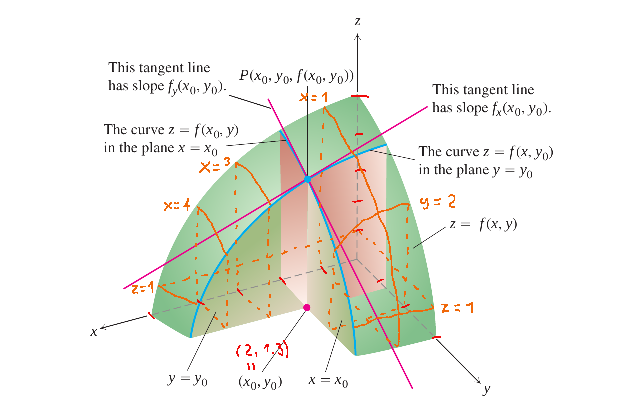
\includegraphics[height=7cm]{2020-2-C3/2021mar24_tomas_gab_1.pdf}





%\printbibliography

\GenericWarning{Success:}{Success!!!}  % Used by `M-x cv'

\end{document}

%  ____  _             _         
% |  _ \(_)_   ___   _(_)_______ 
% | | | | \ \ / / | | | |_  / _ \
% | |_| | |\ V /| |_| | |/ /  __/
% |____// | \_/  \__,_|_/___\___|
%     |__/                       
%
% «djvuize»  (to ".djvuize")
% (find-LATEXgrep "grep --color -nH --null -e djvuize 2020-1*.tex")

 (eepitch-shell)
 (eepitch-kill)
 (eepitch-shell)
# (find-fline "~/2020.2-C3/")
# (find-fline "~/LATEX/2020-2-C3/")
# (find-fline "~/bin/djvuize")

cd /tmp/
for i in *.jpg; do echo f $(basename $i .jpg); done

f () { rm -fv $1.png $1.pdf; djvuize $1.pdf }
f () { rm -fv $1.png $1.pdf; djvuize WHITEBOARDOPTS="-m 1.0" $1.pdf; xpdf $1.pdf }
f () { rm -fv $1.png $1.pdf; djvuize WHITEBOARDOPTS="-m 0.5" $1.pdf; xpdf $1.pdf }
f () { rm -fv $1.png $1.pdf; djvuize WHITEBOARDOPTS="-m 0.25" $1.pdf; xpdf $1.pdf }
f () { cp -fv $1.png $1.pdf       ~/2020.2-C3/
       cp -fv        $1.pdf ~/LATEX/2020-2-C3/
       cat <<%%%
% (find-latexscan-links "C3" "$1")
%%%
}

f 20201213_area_em_funcao_de_theta
f 20201213_area_em_funcao_de_x
f 20201213_area_fatias_pizza



%  __  __       _        
% |  \/  | __ _| | _____ 
% | |\/| |/ _` | |/ / _ \
% | |  | | (_| |   <  __/
% |_|  |_|\__,_|_|\_\___|
%                        
% <make>

 (eepitch-shell)
 (eepitch-kill)
 (eepitch-shell)
# (find-LATEXfile "2019planar-has-1.mk")
make -f 2019.mk STEM=2020-2-C3-MT2 veryclean
make -f 2019.mk STEM=2020-2-C3-MT2 pdf

% Local Variables:
% coding: utf-8-unix
% ee-tla: "c3m202mt2"
% End:
